\documentclass{article}

% Language setting
\usepackage[english]{babel}

% Set page size and margins
\usepackage[letterpaper,top=2cm,bottom=2cm,left=3cm,right=3cm,marginparwidth=1.75cm]{geometry}

% Useful packages
\usepackage{amsmath}
\usepackage{graphicx}
\usepackage[colorlinks=true, allcolors=blue]{hyperref}
\usepackage{float}
\DeclareMathOperator*{\argminA}{arg\,min}

\title{CS461 HW5}
\author{John Bailon}
\date{December 16, 2024}

\begin{document}
\maketitle
\section{EM Algorithm}
\subsection{Log-Likelihood}
A regular Gaussian distribution is represented below

\[\mathcal{N}(\mu, \sigma^2) = \frac{1}{\sqrt{2\pi\sigma^2}}exp(-\frac{(x-\mu)^2}{2\sigma^2})\]

For a Gaussian mixture model, we introduce weight coefficients for each model and their respective mean and variance.

\[f_{X}(x) = \pi_0 \cdot \mathcal{N}(\mu_0, \sigma_0^2) + \pi_1 \cdot \mathcal{N}(\mu_1, \sigma_1^2)\]

To find the log-likelihood for each point, we will first sum the Gaussian probabilities of each model and then take the log.

\[log L = log (\sum_{k} \pi_k \cdot \frac{1}{\sqrt{2\pi\sigma_k^2}}exp(-\frac{(x-\mu_k)^2}{2\sigma_k^2}))\]

Using the code below, I got the following values:

d1: -2.0939

d2: -1.4851

d3: -1.4851

d4: -2.0939

Total log-likelihood: -7.1582

\begin{figure}[H]
    \centering
    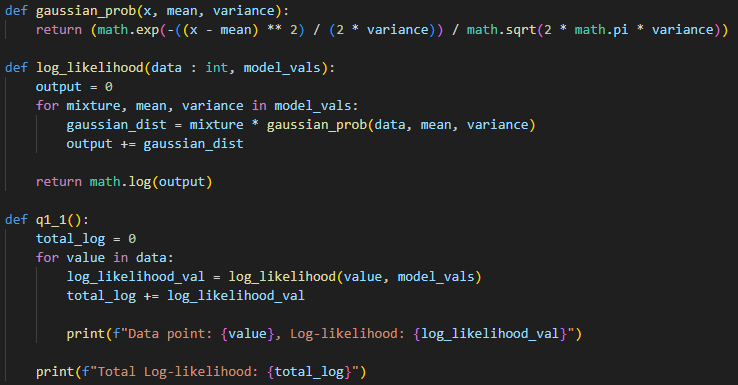
\includegraphics[width=0.8\linewidth]{Q1.1 Code.png}
    \caption{1.1 Code for Log-Likelihood}
\end{figure}

\subsection{E-Step}
For the E-step, we have to calculate the responsibility that each group K assumes for a given data point. The responsibility of group k for point n is given by the following.

\[\gamma_nk = \frac{\pi_k \cdot \mathcal{N}(x_i | \mu_k, \sigma_k^2) }{\sum_{k}\pi_k \cdot \mathcal{N}(x_i | \mu_k, \sigma_k^2)} \]

For each data point, we will calculate the Gaussian probability, multiply it by its weight, and divide by the sum of both models.

Using the code below, I got the following values:

\begin{center}
\begin{tabular}{ c c c }
 Data & $\gamma_0$ & $\gamma_1$ \\
 d1 & 0.0180 & 0.9820 \\ 
 d2 & 0.1192 & 0.8808 \\  
 d3 & 0.8808 & 0.1192 \\
 d4 & 0.9820 & 0.0180 \\  
\end{tabular}
\end{center}

\begin{figure}[H]
    \centering
    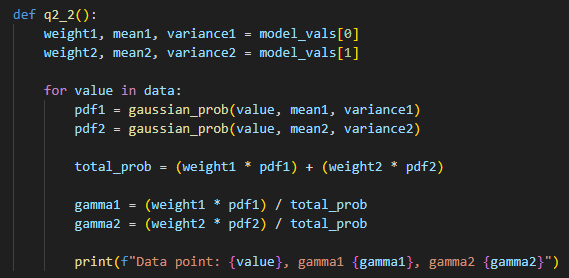
\includegraphics[width=0.75\linewidth]{Q1.2 Code.png}
    \caption{1.2 Code for E-Step}
\end{figure}

\subsection{M-Step}
Finally, we will update the parameters, weight coeff, mean, and variance for each model. 

The weight is updated using:

\[\pi_k(t+1) = \frac{\sum_{n}\gamma_{nk}(\theta_t)}{N} \]

\[\pi_0(t+1) = \pi_1(t+1) = \frac{0.0180+0.1192+0.8808+0.9820}{4} = \frac{1}{2} \]

The mean is updated using:

\[\mu_k(t+1) = \frac{\sum_N \gamma_{nk} * x_n}{\sum_N \gamma_{nk}} \]

The variance is updated using:

\[\sigma_k^2(t+1) = \frac{\sum_N \gamma_{nk} * (x_n - \mu_k)^2 }{\sum_N \gamma_{nk}} \]

Using the code below, I got the following values:
\begin{figure}
    \centering
    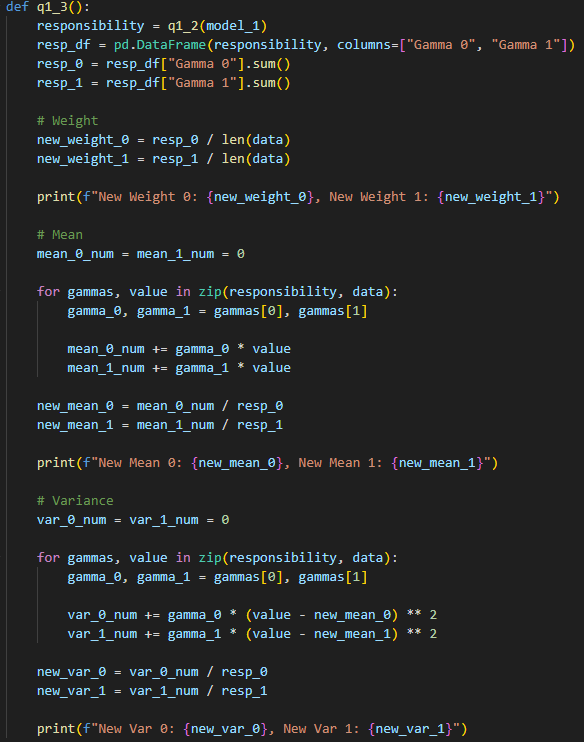
\includegraphics[width=0.5\linewidth]{Q1.3 Code.png}
    \caption{1.3 Code for M-Step}
\end{figure}

\begin{center}
\begin{tabular}{ c c c }
 Parameter & Model 0 & Model 1 \\
 $\pi$      & 0.5 & 0.5 \\ 
 $\mu$      & -1.3448 & 1.3448 \\  
 $\sigma^2$ & 0.6914 & 0.6914 \\
\end{tabular}
\end{center}

\subsection{Updated Log-likelihood}
Using the values found in 1.3 and the code from 1.1, I recomputed the log-likelihood below. The total log-likelihood has increased.

d1: -1.7376 

d2: -1.4933 

d3: -1.4933 

d4: -1.7376 

Total log-likelihood: -6.4619

\section{Exact v. Approximate inference}
\subsection{Variable Elimination}
Using the structure of the provided network and conditional probability and marginalization, we have:

\[ P(Cloudy | Sprinkler = T, WetGrass = T) = \alpha\sum_{rain} P(Cloudy, Sprinkler, Rain, Wet Grass)\]

We will use normalization later to find the posterior probability. Next, we substitute the joint probability for its Bayesian network representation

\[ = \alpha \sum_{rain} P(Cloudy) * P(Sprinkler | Cloudy) * P(Rain | Cloudy) * P(WetGrass | Sprinkler, rain)\]

\[ = \alpha * P(Cloudy) * P(Sprinkler | Cloudy) \sum_{rain} P(Rain | Cloudy) * P(WetGrass | Sprinkler, rain)\]

For Cloudy = T

\[ = \alpha * 0.5 * 0.1 * ((0.8 * 0.99) + (0.2 * 0.9))\]
\[ = 0.0486\alpha\]

For Cloudy = F

\[ = \alpha * 0.5 * 0.5 * ((0.2 * 0.99) + (0.8 * 0.9))\]
\[ = 0.2295\alpha\]

Finally, normalize

\[P(Cloudy | Sprinkler = T, WetGrass = T) = \frac{0.0486}{0.0486 + 0.2295} = 17.48 \%\]

\subsection{Gibbs Sampling}
For Gibbs sampling, we will assign all variables in the network to arbitrary values, fixing the evidence variables, sprinkler, and wet grass, to true. Next, we will generate samples for both cloudy and rainy by calculating their probability conditional on their Markov blankets. The general form is

\[ P(Target | Markov Blanket) = \alpha P(Target | Parent) * P(Children | Coparent and Target)\]

For Cloudy:
\[ P(Cloudy | Sprinkler, Rainy) = \alpha P( Cloudy) * P(Sprinkler | Cloudy) * P(Rainy | Cloudy)\]

For Rainy:
\[ P(Rainy | Cloudy, wetgrass, Sprinkler) = \alpha P(Rainy | Cloudy) * P(WetGrass | Sprinkler, Rainy)\]

We will assign cloudy and rainy based on the computed probability and repeat. The mean of the generated sample will approximate the prior.

Below is the code I used to solve this problem. After 1,000,000 iterations, the prior is estimated to be 17.53\%.

\begin{figure}[H]
    \centering
    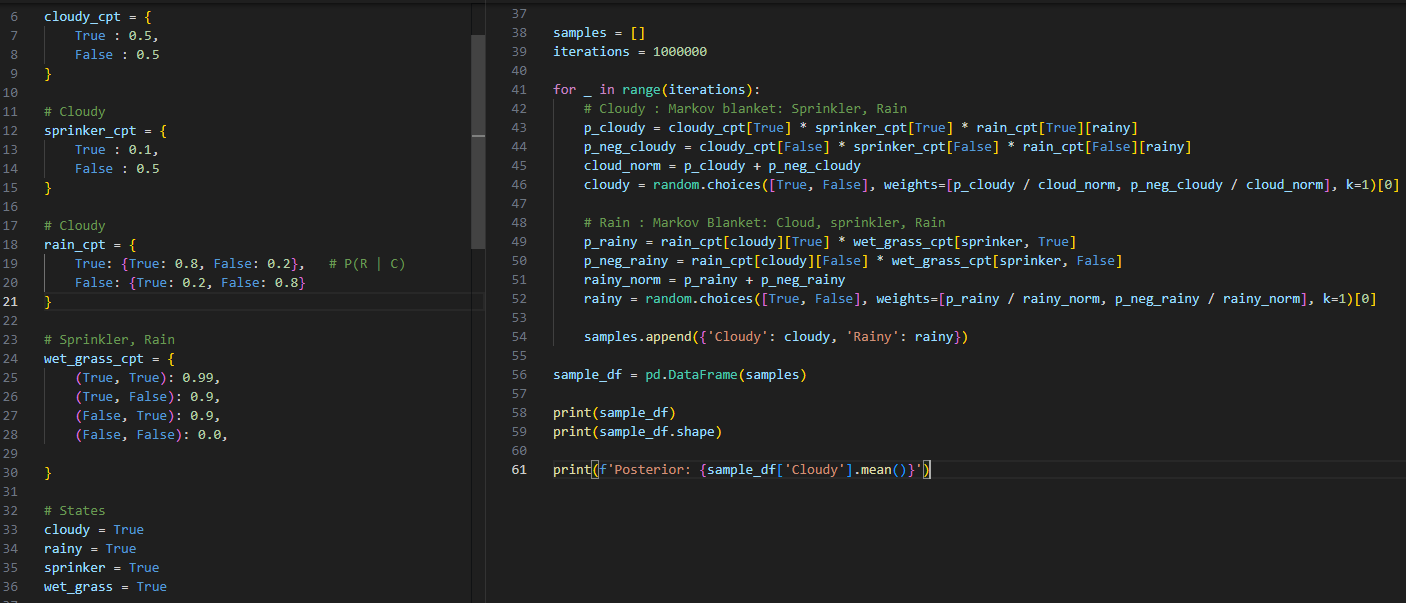
\includegraphics[width=1\linewidth]{Q2 Code.png}
    \caption{2.2 Gibbs Sampling Implementation}
    \label{fig:enter-label}
\end{figure}

\section{VAE Lower Bound (ELBO)}
\subsection{Derive the Inequality}

First we start with the marginal log-likelihood:

\[\log P_\theta (x_i) = log \sum_z  P_\theta(x_i, Z) \]

Next, we add an approximate posterior by multiplying and dividing,

\[ = log \sum_z   q_\phi (Z | x_i) *\frac{P_\theta(x_i, Z) }{q_\phi (Z | x_i)} \]
\[ = log E_{q_\phi (Z | x_i)}[\frac{P_\theta(x_i, Z) }{q_\phi (Z | x_i)}]\]

Next, we use Jensen's inequality, which states:

\[E[\log X] \leq \log E[X]\]

We can rewrite the above as an inequality,

\[ \geq E_{q_\phi (Z | x_i)} [log\frac{P_\theta(x_i, Z) }{q_\phi (Z | x_i)}]\]

Next, manipulate the equation using log properties,

\[ \geq E_{q_\phi (Z | x_i)} [log (P_\theta(x_i, Z)) - log (q_\phi (Z | x_i))]\]

Expand the joint probability, $P_\theta(x_i, Z)$ and once again use log properties

\[ \geq E_{q_\phi (Z | x_i)} [log (P_\theta(x_i | Z)) + log(P_\theta(Z)) - log (q_\phi (Z | x_i))]\]

Expand the terms within the expected value, and factor out -1 from the last two terms

\[ \geq E_{q_\phi (Z | x_i)} [log (P_\theta(x_i | Z))] - E_{q_\phi (Z | x_i)}[log (q_\phi (Z | x_i)) - log(P_\theta(Z))]\]

Here we can substitute the second term for the KL divergence and reorder to complete the proof.

\[ = - D_{KL}q_\phi(z|x_i) || p_\theta(z) + E_{q_\phi (Z | x_i)} [log (P_\theta(x_i | Z))] )\]

\section{RBM Movie Recommendation System}
\subsection{Bipolar Coding}
The RBM in Figure 2 represents a recommendation system that encodes the preference for movies. A binary coding is not sufficient for this system as it needs to encode both like and dislike of a movie. Thus, a bipolar coding is more appropriate as like and dislike can be represented by positive and negative values, and unwatched movies can be represented with zeroes.

\subsection{Modify RBM Conditional Probability}
The derived conditional probability does not work as the sigmoid function ranges from 0 to 1. Since we are using a bipolar coding, we need our function to range from -1 to 1.

We follow the same derivation as in class. However, instead of normalizing with h = 0, we must normalize with h = -1.

\[P(h=1 | m1, m2, m3 = \alpha\cdot exp (m^t W[:,1] + C_1)\]
\[P(h=-1 | m1, m2, m3 = \alpha\cdot exp (-m^t W[:,1] + C_1)\]

Normalizing these functions we can use hyperbolic identities to derive
\[P(h=1 | m1, m2, m3 = \frac{1+\tanh{exp (m^t W[:,1] + C_1)}}{2}\]

\[P(m=1 | m1, m2, m3 = \frac{1+\tanh{exp (W[1,:]h + b_1)}}{2}\]

\subsection{Predict Movie Preference}
\end{document}